\documentclass[12pt,letterpaper,oneside,reqno]{amsart}
\usepackage{amsfonts}
\usepackage{amsmath}
\usepackage{amssymb}
\usepackage{amsthm}
\usepackage{float}
\usepackage{mathrsfs}
\usepackage{colonequals}
\usepackage[font=small,labelfont=bf]{caption}
\usepackage[left=1in,right=1in,bottom=1in,top=1in]{geometry}
\usepackage[pdfpagelabels,hyperindex,colorlinks=true,linkcolor=blue,urlcolor=magenta,citecolor=green]{hyperref}
\usepackage{graphicx}
\linespread{1.7}
\emergencystretch=1em
\usepackage{array}
\usepackage{etoolbox}
\apptocmd{\sloppy}{\hbadness 10000\relax}{}{}
\raggedbottom

\newcommand \anglePower [2]{\langle #1 \rangle \sp{#2}}
\newcommand \bernoulli [2][B] {{#1}\sb{#2}}
\newcommand \curvePower [2]{\{#1\}\sp{#2}}
\newcommand \coeffA [3][A] {{\mathbf{#1}} \sb{#2,#3}}
\newcommand \polynomialP [4][P]{{\mathbf{#1}}\sp{#2} \sb{#3}(#4)}

% ordinary derivatives
\newcommand \derivative [2] {\frac{d}{d #2} #1}                              % 1 - function; 2 - variable;
\newcommand \pderivative [2] {\frac{\partial #1}{\partial #2}}               % 1 - function; 2 - variable;
\newcommand \qderivative [1] {D_{q} #1}                                      % 1 - function
\newcommand \nqderivative [1] {D_{n,q} #1}                                   % 1 - function
\newcommand \qpowerDerivative [1] {\mathcal{D}_q #1}                         % 1 - function;
\newcommand \finiteDifference [1] {\Delta #1}                                % 1 - function;
\newcommand \pTsDerivative [2] {\frac{\partial #1}{\Delta #2}}               % 1 - function; 2 - variable;

% high order derivatives
\newcommand \derivativeHO [3] {\frac{d^{#3}}{d {#2}^{#3}} #1}                % 1 - function; 2 - variable; 3 - order
\newcommand \pderivativeHO [3]{\frac{\partial^{#3}}{\partial {#2}^{#3}} #1}
\newcommand \qderivativeHO [2] {D_{q}^{#2} #1}                               % 1 - function; 2 - order
\newcommand \qpowerDerivativeHO [2] {\mathcal{D}_{q}^{#2} #1}                % 1 - function; 2 - order
\newcommand \finiteDifferenceHO [2] {\Delta^{#2} #1}                         % 1 - function; 2 - order
\newcommand \pTsDerivativeHO [3] {\frac{\partial^{#3}}{\Delta {#2}^{#3}} #1} % 1 - function; 2 - variable;
\newcommand{\stirlingii}{\genfrac{\{}{\}}{0pt}{}}
\newcommand{\eulerianNumber}{\genfrac{\langle}{\rangle}{0pt}{}}

\newtheorem{thm}{Theorem}[section]
\newtheorem{cor}[thm]{Corollary}
\newtheorem{lem}[thm]{Lemma}
\newtheorem{examp}[thm]{Example}
\newtheorem{conj}[thm]{Conjecture}
\newtheorem{defn}[thm]{Definition}

\numberwithin{equation}{section}

\title[Polynomial identities involving Central Factorial numbers]
{Polynomial identities involving Central Factorial numbers}
\author[Petro Kolosov]{Petro Kolosov}
\email{kolosovp94@gmail.com}
\keywords{
    Polynomials,
    Polynomial identities,
    Faulhaber's formula,
    Cental Factorial Numbers
}
\urladdr{https://kolosovpetro.github.io}
\subjclass[2010]{26E70, 05A30}
\date{\today}
\hypersetup{
    pdftitle={Polynomial identities involving Central Factorial numbers},
    pdfsubject={
        Polynomials,
        Polynomial identities,
        Faulhaber's formula,
        Cental Factorial Numbers
    },
    pdfauthor={Petro Kolosov},
    pdfkeywords={
        Polynomials,
        Polynomial identities,
        Faulhaber's formula,
        Cental Factorial Numbers
    }
}
\begin{document}
    \begin{abstract}
        Your abstract here.
    \end{abstract}

    \maketitle

    \tableofcontents


    \section{Introduction} \label{sec:introduction}
    Your introduction here.
Include some references~\cite{bayour2017truly,benkhettou2016conformable,caputo2009time,martins2009calculus,
    GithubSource_2022, Sloane_theencyclopedia}.
Lorem Ipsum is simply dummy text of the printing and typesetting industry.
Lorem Ipsum has been the industry's standard dummy text ever since the 1500s, when an unknown printer took a galley
of type and scrambled it to make a type specimen book.
It has survived not only five centuries, but also the leap into electronic typesetting, remaining essentially unchanged.
It was popularised in the 1960s with the release of Letraset sheets containing Lorem Ipsum passages, and more
recently with desktop publishing software like Aldus PageMaker including versions of Lorem Ipsum.

Figure example
\begin{figure}[H]
    \centering
    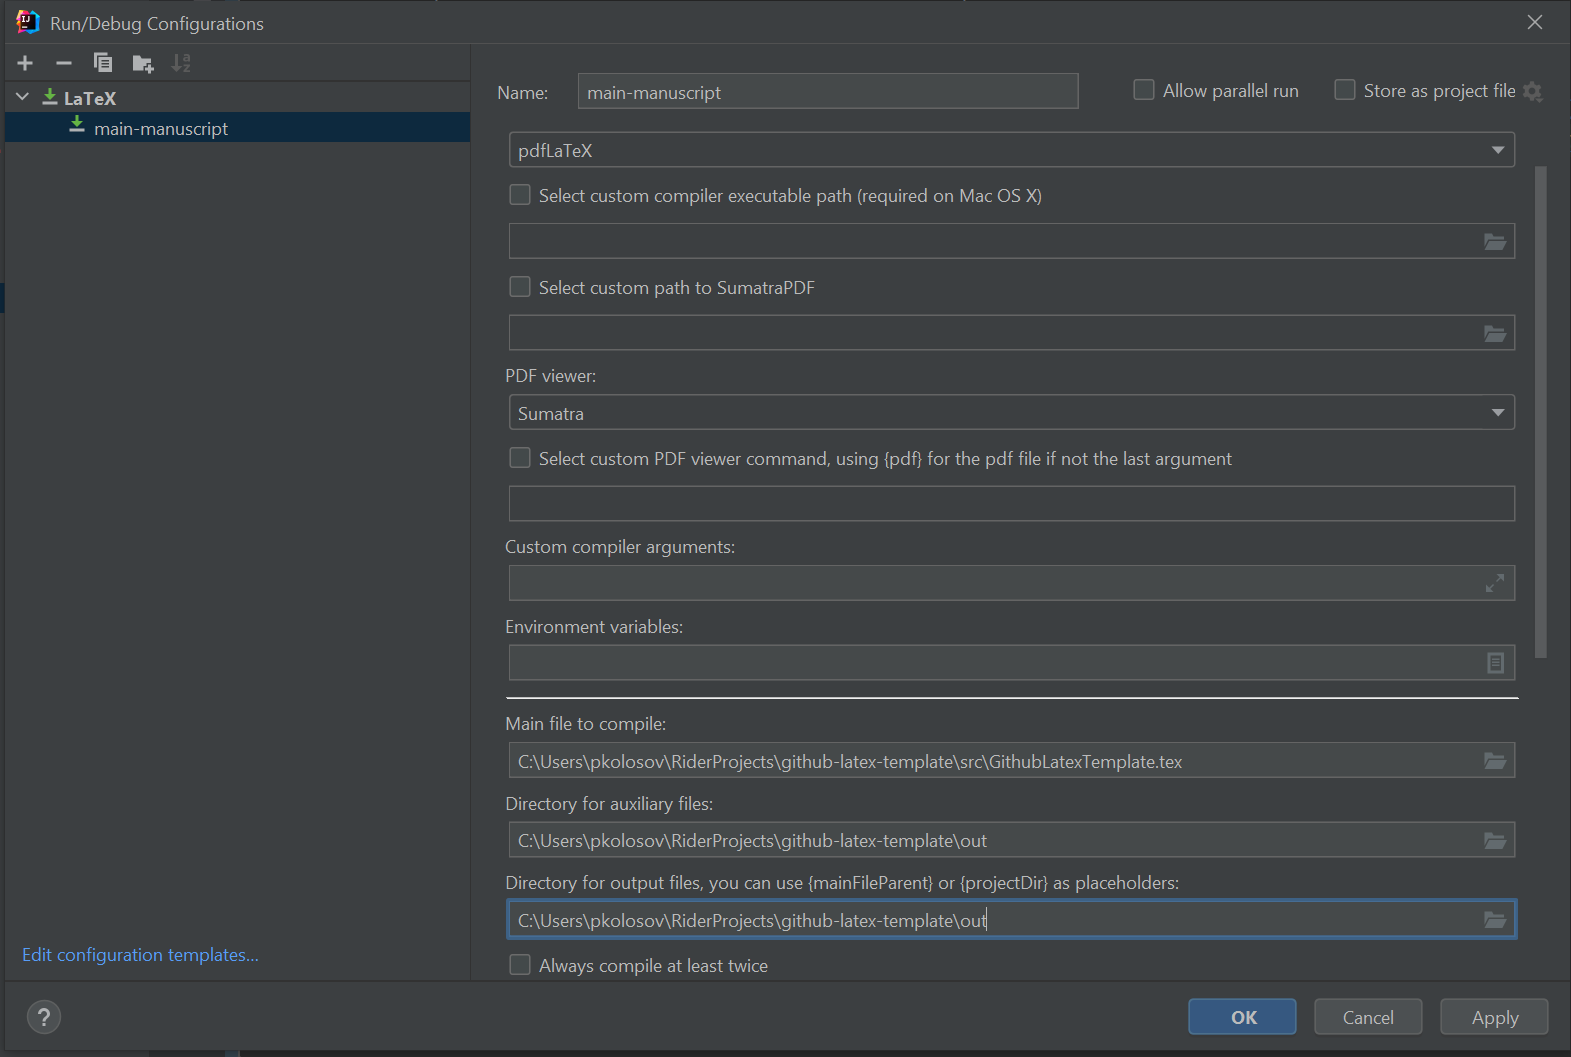
\includegraphics[width=1\textwidth]{../img/latex_configuration}
    ~\caption{Figure example.}\label{fig:figure}
\end{figure}


    \section{Conclusions}\label{sec:conclusions}
    Conclusions of your manuscript.

    \bibliographystyle{unsrt}
    \bibliography{PolynomialIdentitiesInvolvingCentralFactorialNumbers}
    \noindent \textbf{Version:} \texttt{Local-0.1.0}

\end{document}
